\documentclass[11pt,a4paper]{article}
\usepackage[margin=2.5cm]{geometry}
\usepackage{amsmath,amssymb}
\usepackage{booktabs}
\usepackage{graphicx}
\usepackage{tikz}
\usetikzlibrary{arrows.meta,positioning,fit,backgrounds}
\usepackage[colorlinks=true,linkcolor=blue!50!black,citecolor=blue!50!black,urlcolor=blue!50!black]{hyperref}
\usepackage{microtype}
\usepackage{seqsplit}
\newcommand{\longhash}[1]{\texttt{\footnotesize\seqsplit{#1}}}
\usepackage{xcolor}
\usepackage{enumitem}
\setlist{nosep,leftmargin=1.4em}
\usepackage[round]{natbib}
\bibliographystyle{plainnat}

\newcommand{\code}[1]{\texttt{\small #1}}
\newcommand{\sha}[1]{\texttt{\scriptsize #1}}
\newtheorem{observation}{Observation}
\newtheorem{proposition}{Proposition}

\title{\bfseries Reproducing the verification record of a\\ computer-assisted proof:\\[2pt]
the dimension-six MUB preprint, the covering step,\\ and what the prose determines}
\author{MUB-6 Reconstruction Project\thanks{Produced by a six-team agent programme running in an
Open Math OS environment on 14 November 2026. All code, logs and hashes cited here are in the
accompanying \code{mub6-recreate/} directory.}}
\date{14 November 2026}

\begin{document}
\maketitle

\begin{abstract}
\noindent
The preprint \emph{The maximum number of mutually unbiased bases in dimension six}
\citep{OpenAIMUB2026} claims $N(6)=3$ by a computer-assisted argument, and publishes its verification
material: seven C++ sources (2\,265 lines), four programs, a 100-command execution record and 82.3\,MB of
recorded numerical data. We report an independent reproduction of the first
of its programs --- the \emph{covering step}, which turns a 112-bin seed enumeration into 249\,878
covering centres --- and of the record's verification apparatus.

Our build reproduces the recorded \code{centers.txt} \emph{byte for byte} (7\,339\,546 bytes,
SHA-256 \sha{c48bc9a2\ldots789}), and reproduces every one of the program's five internal counters
(151\,744\,086 pair tests, 29\,769\,262\,282 bucket visits, 3\,134\,060\,273 linear programs), so the
agreement extends to every decision taken and not merely to the surviving rows. A second,
independently written implementation agrees. The two are silent about nothing: the arithmetic core is
bit-identical to the published source over a 66\,204\,081-byte dump, and the interval tests have a
minimum slack of $1.043\times10^{-9}$ over $4.74\times10^{9}$ trials, so this stage has no
knife-edge.

A clean-room reconstruction from the manuscript alone recovers the seed \emph{set} exactly (22\,829,
matching the count the record prints) but not its \emph{order}: of the 120 loop nestings exactly one
reproduces the record, the natural reading permutes 5\,497 of the 249\,878 lines, and the count is
blind to the difference. The manuscript's prose is therefore sufficient for the numbers it quotes and
insufficient for the file it distributes.

Three properties of the published apparatus are worth reporting. Its per-command transcripts are
curated, not raw stdout, and cannot be regenerated by the programs that produced the run. Its command
manifest omits two families of output. And its checker cannot detect an in-bounds alteration of a
parent record, because nothing compares a parent's bytes with the children derived from it. We claim
nothing about the theorem itself, and the remaining three stages are not re-derived here.
\end{abstract}

\tableofcontents

\section{Introduction}

For $d$ a prime power the maximum number $N(d)$ of mutually unbiased bases (MUBs) in $\mathbb{C}^d$ is
known to be $d+1$ \citep{Ivanovic1981StateDetermination,WoottersFields1989,BandyopadhyayEtAl2002,
KlappeneckerRotteler2004}. For $d=6$ --- the smallest dimension that is not a prime power --- three
bases are classical and the existence of a fourth is the subject of a long-standing conjecture that
$N(6)=3$; see \citet{Zauner1999,Zauner2011} and the review \citep{McNultyWeigert2026Review}. Numerical
and algebraic evidence has accumulated for two decades
\citep{ButterleyHall2007Numerical,BrierleyWeigert2008,BrierleyWeigert2009,JamingEtAl2009,
JamingMatolcsiMora2010,BengtssonEtAl2007MUBHadamard,Grassl2004SICMUB6,
CardenesWuttigTindall2026Classification,MatolcsiEtAl2026}.

The preprint \citep{OpenAIMUB2026} (76 pages, 24 September 2026) claims a proof of $N(6)=3$ by a
computer-assisted argument, conditional on a documented binary64 arithmetic contract and on one
recorded execution. It is unusual in publishing not only the argument but the machinery: seven C++
sources, a build script that compiles four programs, an arithmetic/ABI probe, a record checker, and
the complete numerical output of the run that the proof invokes. A formal component accompanies the
paper; it establishes a weaker bound, not $N(6)=3$.

Published code and published output together make a stronger kind of check possible than either
alone. One can ask not merely ``is the record internally consistent?'' --- which the authors' own
checker answers --- but ``does an implementation written from the specification reproduce the record,
down to the last byte and the last counter?'' That question has a sharp answer, and when the answer is
yes it localises any future disagreement to the specification rather than to the run.

This paper reports such an exercise for the first of the four programs. The scope is deliberately
narrow, and we state it at the outset so that no reader mistakes what follows for a verification of
the theorem.

\begin{enumerate}[label=(\roman*)]
\item We re-derived the covering step --- \code{seed.cpp} (119 lines) and \code{covout.cpp}
(143 lines), which enumerate the seeds on a 112-fraction grid and select 249\,878 covering centres ---
behind a frozen interface, twice, by two independent implementations. Both reproduce the recorded
\code{centers.txt} byte for byte and all five of its counters.
\item We measured what the manuscript alone determines, by rebuilding the seed enumeration from the
prose without reading the sources. The set is determined; the order is not.
\item We examined the published verification apparatus and report three properties that a reader of
the preprint should know.
\end{enumerate}

We do \emph{not} re-derive the three refinement stages (programs \code{arun}, \code{brun},
\code{crun}), do not re-run the 100-command pipeline with our own build, and make no claim about
$N(6)$.

\section{The published record}\label{sec:record}

\subsection{Sources and programs}
The mathematics is carried by seven files, \code{seed.cpp} \code{ub.cpp} \code{patchx.cpp}
\code{atlas.cpp} \code{stageB.cpp} \code{stageC.cpp} \code{covout.cpp}, 2\,265 lines in total, plus a
51-line arithmetic probe. They are not separate translation units: \code{stageC.cpp} includes
\code{stageB.cpp} includes \code{atlas.cpp} includes \code{patchx.cpp} includes \code{ub.cpp}
includes \code{seed.cpp}, each file defining the next file's include guard and hiding its own
\code{main} behind it. Four programs are built: \code{covrun} (from \code{covout.cpp}), \code{arun},
\code{brun}, \code{crun}. Three further \code{main}s exist in the sources and are never built.

Table~\ref{tab:files} lists the files with their hashes as published. The seven mathematical sources
match the hashes in the package's own extraction manifest, so the object of reproduction is
unambiguous.

\begin{table}[t]
\centering\small
\caption{The published sources. Lines and bytes are as distributed; hashes are SHA-256, truncated.
The seven mathematical files match \code{verification/code/extraction.json}.}
\label{tab:files}
\begin{tabular}{lrrl}
\toprule
file & lines & bytes & SHA-256 (first 12) \\
\midrule
\code{seed.cpp}    & 119 & 3\,514  & \sha{3c6c7a709223} \\
\code{ub.cpp}      & 386 & 11\,557 & \sha{bb0312823400} \\
\code{patchx.cpp}  & 473 & 16\,137 & \sha{a78a1ab171d8} \\
\code{atlas.cpp}   & 241 & 8\,821  & \sha{dcbf2dbe1054} \\
\code{stageB.cpp}  & 336 & 12\,030 & \sha{7e609a2f282d} \\
\code{stageC.cpp}  & 567 & 17\,471 & \sha{60a1b1009185} \\
\code{covout.cpp}  & 143 & 5\,286  & \sha{2a7e6bf5ca48} \\
\midrule
\code{abi-fp-probe.cpp} & 51 & 2\,496 & (not in manifest) \\
\code{build.sh}         & 29 & 1\,303 & --- \\
\code{check\_records.py} & 373 & 18\,229 & --- \\
\bottomrule
\end{tabular}
\end{table}

The build is pinned by flags as much as by sources: \code{g++ -O3 -march=native -ffp-contract=off}
for the first two programs and \code{-std=gnu++17} added for the rest, with \code{LANG=C}. The probe
refuses to compile under a fast-math mode and requires binary64 with round-to-nearest, gradual
underflow, no FTZ/DAZ and \code{FLT\_EVAL\_METHOD == 0} \citep{IEEE7542019,Higham2002Accuracy}.

\begin{figure}[t]
\centering
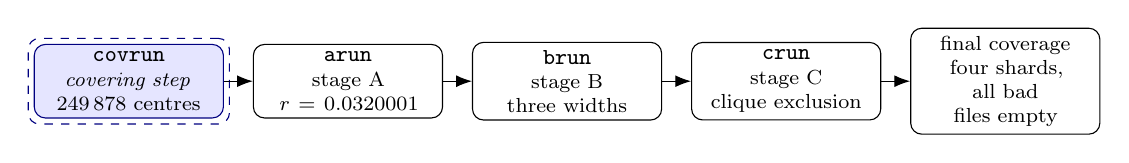
\begin{tikzpicture}[scale=0.92,transform shape,
  box/.style={draw,rounded corners,align=center,font=\footnotesize,minimum height=10mm,inner sep=3pt,text width=24mm},
  rep/.style={box,fill=blue!10,draw=blue!50!black},
  ar/.style={-{Latex[length=2mm]}}]
\node[rep] (cov) {\code{covrun}\\ \emph{covering step}\\ 249\,878 centres};
\node[box,right=4mm of cov] (a) {\code{arun}\\ stage A\\ $r=0.0320001$};
\node[box,right=4mm of a] (b) {\code{brun}\\ stage B\\ three widths};
\node[box,right=4mm of b] (c) {\code{crun}\\ stage C\\ clique exclusion};
\node[box,right=4mm of c] (f) {final coverage\\ four shards, all bad\\ files empty};
\draw[ar] (cov)--(a); \draw[ar] (a)--(b); \draw[ar] (b)--(c); \draw[ar] (c)--(f);
\begin{scope}[on background layer]
\node[draw=blue!50!black,dashed,rounded corners,fit=(cov),inner sep=2pt] {};
\end{scope}
\end{tikzpicture}
\caption{The recorded pipeline. The shaded program is the one reproduced here, together with the
seed enumeration that feeds it; the three refinement stages and the final coverage certificate are
not re-derived in this report. Stage B runs three times --- at $.07/.013$, at $.016/.005$ (batched),
and at $.011/.0038$ over the batches that stage C left unresolved.}
\label{fig:pipeline}
\end{figure}

\subsection{The run and its artefacts}
The recorded execution is a 100-command DAG, given in \code{commands.json} with argv, inputs, outputs
and return codes: one \code{covrun}; four \code{arun} invocations partitioning the centres modulo 4;
one \code{brun} at target/width $.07/.013$; one \code{brun} at $.016/.005$ which emits 88 batches of
at most 256 records; 88 \code{crun} invocations, one per batch; one \code{brun} at $.011/.0038$ over
the 15 batches that reported unresolved records; and four \code{crun} invocations partitioning the
fallback output modulo 4. Of the 100 commands, 85 return 0 and 15 return 1 --- the 15 being exactly
the batches with unresolved records, which the fallback then re-refines. An empty final bad file is
the proof that the coverage completed.

The numerical data total 193 files and 82\,327\,335 bytes (Table~\ref{tab:artefacts}); the
transcripts add 30\,768 bytes in 100 files. Figure~\ref{fig:pipeline} shows where the covering step
sits and where this report stops.

\begin{table}[t]
\centering\small
\caption{Artefacts produced by the recorded run. Record files are little-endian: a \code{uint64}
count, then per record \code{int k}, \code{double p[36]}, \code{double T[k][36]} and eight doubles.}
\label{tab:artefacts}
\begin{tabular}{llrl}
\toprule
family & produced by & files & bytes \\
\midrule
\code{centers.txt} & \code{covrun} & 1 & 7\,339\,546 \\
\code{coarse0..3.bin} & \code{arun} (4 parts) & 4 & 4\,644\,588 \\
\code{mid.bin} & \code{brun} $.07/.013$ & 1 & 903\,656 \\
\code{fine.bin} & \code{brun} $.016/.005$ & 1 & 33\,746\,388 \\
\code{batches/f*.bin} & the same run, batched & 88 & 33\,747\,084 \\
\code{batches/bad*.bin} & \code{crun} (88) & 88 & 246\,508 \\
\code{fb1.bin} & \code{brun} $.011/.0038$ & 1 & 1\,699\,524 \\
\code{fb1cbad0..3.bin} & \code{crun} (4 parts) & 4 & 32 \\
\code{bad0..3.txt} & \code{arun} & 4 & 0 \\
\code{batches/fdone.txt} & \code{brun} & 1 & 9 \\
\midrule
numerical data & & 193 & 82\,327\,335 \\
transcripts & all commands & 100 & 30\,768 \\
\bottomrule
\end{tabular}
\end{table}

\section{Method}\label{sec:method}

\subsection{A frozen interface, then two implementations}
Work began by writing down every contract the record depends on and that the sources fix: program
arguments and their enforced ranges, the two on-disk formats, the constants, the exit-code semantics,
the module boundary, and a \emph{determinism register} of 29 order- or rounding-carrying constructs.
That document was frozen before any code was written and then attacked adversarially; it accumulated
32 findings, several of them errors in the document rather than in the code. The two that mattered
most: the cover's bucket grid is $K=\lfloor Rn+0.51\rfloor=4$ with $m=\lceil n/K\rceil=28$, not the $3/38$ a hand computation had written
down; and the dephasing used in every record read is $p_{ij}-p_{i0}-p_{0j}+p_{00}$, in which writing
$p_{0j}$ as \code{p[6j]} transposes the column term.

Two implementations were then written independently against that contract --- one split into five
translation units, one into two --- and each was checked against the recorded artefact rather than
against the other.

\subsection{How the work was organised}
The exercise was run as six agent teams with disjoint write scopes: coding; verification (harness and
logs, never algorithm code); critics (read-only, every finding required to name the test that would
settle it); documentation; summarisation; and a desk that owns the frozen contract, the change
requests and the gates. The programme produced 32 findings against the contract before a line of code
was judged. Four of them were errors in the contract
itself --- the bucket grid, the dephasing transpose, the batch-radius rewrite and the enumeration
order --- and each of those would independently have produced a plausible-looking artefact that
failed byte identity. The separation of the critic role from the coding role is what made that cheap:
the critic had no stake in the code and no permission to fix it.

\subsection{A ladder, and controls that can fail}
Reproduction is graded by rungs: R0 the arithmetic/ABI contract on the build host; R1 unit tests
written against exact values rather than against our own output; R2 the covering file byte-identical;
R3--R6 the four refinement families and finally the full 100-command replay with return codes. This
paper reports R0--R2.

Because a differential harness passes by construction when it compares an artefact with itself, the
harness is required to fail on planted defects. Twelve seeded corruptions --- a flipped byte, an
appended byte, a truncation, a swapped double, a perturbed return code, a dropped record, a wrong
count, an out-of-range radius, a wrong batch marker, a non-empty \code{arun} bad file, a permuted
fallback order, a nonzero final bad count --- are all caught, each by a named check. The check that
detects an appended byte is not the check that detects a permuted fallback order, which is the point.

\section{The covering step reproduced}\label{sec:results}

\subsection{What the program does}
\code{covrun} enumerates seeds on the grid $\{0,\tfrac1{112},\ldots\}$: weakly increasing five-tuples
of bins, filtered by two gap inequalities and by an interval test for whether a certain point lies in
a certain polygon. It then selects a subset of \emph{centres} --- pairs (seed, five-bin tail) --- such
that every admissible pair is within $R=0.032$ of a selected one, in a norm whose unit ball is a
hexagon, using a bucketed search with a dual (linear-programming) bound for the pairs the cheap test
cannot decide. The output is 249\,878 centres.

\subsection{Byte identity, and more}
Our build writes 7\,339\,546 bytes whose SHA-256 equals the recorded file's:
\begin{center}\longhash{c48bc9a2be1eb2cdeea82ea1b030d7cb9f00a6c9563b63f0248dd115748a5789}\end{center} A format audit confirms the
details that a naive comparison would miss: ten decimal fields per row, each followed by a space, no
carriage returns, one trailing space before the newline, 13\,557 contiguous blocks.

Byte identity of the output is weaker than it sounds, because the covering step could in principle
reach the same set of centres by a different route. We therefore also compared the program's five
internal counters, which count decisions rather than outputs
(Table~\ref{tab:counters}). All five agree.

\begin{table}[t]
\centering\small
\caption{Internal counters. The published build was compiled from the distributed sources with
\code{build.sh}; ours from \code{mub6-recreate/src}. Agreement on \code{visit} and \code{lp} means the
bucket scan order, the cheap tests and the dual bound all agree, not merely the surviving centres.}
\label{tab:counters}
\begin{tabular}{lrr}
\toprule
counter & published build & our build \\
\midrule
\code{checked} pairs & 151\,744\,086 & 151\,744\,086 \\
\code{centers}       & 249\,878     & 249\,878 \\
\code{visit}         & 29\,769\,262\,282 & 29\,769\,262\,282 \\
\code{near}          & 3\,341\,641\,851 & 3\,341\,641\,851 \\
\code{cheap}         & 45\,648\,766 & 45\,648\,766 \\
\code{lp}            & 3\,134\,060\,273 & 3\,134\,060\,273 \\
\midrule
wall clock & 401.8\,s & 400.8\,s \\
\bottomrule
\end{tabular}
\end{table}

\subsection{The arithmetic core, bit for bit}
The enumeration's arithmetic is the delicate part: the exponential is evaluated by a degree-nine
polynomial with quadrant reduction rather than by \code{libm}, and the interval test carries a
coefficient of $5\pi/(4N^2)$ and a $10^{-8}$ slack. We compared a dump of the entire seed structure
--- $n$, $w$, $\pi$, 112 table entries, all 22\,829 seeds with their skip index, gap and both centre
coordinates, and all 829\,306 tails --- against a probe that includes the distributed
\code{seed.cpp} verbatim. The two dumps are identical: 66\,204\,081 bytes, SHA-256
\sha{7fb12e3b\ldots}.

Two further measurements bear on the binary64 contract, which the preprint's Theorem~1.1 is
conditional on:
\begin{itemize}
\item the computed coefficient is $3.13057303650130804538\times10^{-4}$, which is exactly
$5\pi/(4\cdot112^2)$ as a real number rounded to binary64 minus nothing --- it is $0.00$ ulp from the
correctly rounded value;
\item over $4.74\times10^{9}$ interval tests, the minimum absolute slack is $1.043\times10^{-9}$. The
test is nowhere near a tie, so a rounding difference of one ulp cannot flip a decision at this stage.
\end{itemize}

The second fact is the more interesting one: it says that this stage of the record is robust to the
arithmetic contract it is embedded in, which is not something one can assume and not something the
manuscript states. A third instance of the same insensitivity sits in the covering code: its two
square terms compile to calls to the library \code{pow} rather than to multiplications, and at both
actual arguments $\code{pow}(v,2)$ and $v\cdot v$ agree bit for bit --- though they differ by one ulp
on about $4.5\times10^{-4}$ of random arguments, so this is luck at two points rather than a general
identity.

\subsection{Two implementations, and the cost of modularity}
The two implementations differ in translation-unit structure (five units and two units) and in
internal organisation, and were written by different agents from the same frozen contract. Both
reproduce the file and all counters.

A third build, compiled at \code{-O2} with no \code{-march=native}, also reproduces the recorded file
byte for byte (623\,s against 524\,s for the faithful build). Byte identity here is therefore not
fragile to the compiler flags, which is worth knowing for anyone who wants to rerun this on other
hardware --- and is a fact about this stage only.

We expected that splitting the single translation unit would change code generation and break
identity. It did not. We then measured that the split costs $1.9\times$ (759.6\,s against
401.8\,s) --- and that measurement was wrong, taken while thirteen agents shared four CPUs. Re-measured
on an idle machine, the modular build takes 400.8\,s against the published 401.8\,s. There is no
detectable penalty, because the hot loops are already self-contained. We record the correction because
it is the kind of claim that is cheap to make and expensive to be wrong about.

\section{What the prose determines}\label{sec:cleanroom}

The record exists to support a proof, so the interesting question is not only whether the code
reproduces the file but whether the \emph{paper} does. We rebuilt the seed enumeration from the
manuscript alone --- Section 2 and Appendix A.2--A.3 --- without opening \code{seed.cpp} or
\code{covout.cpp}, and compared the result with the record.

\paragraph{The set is determined.} The prose yields exactly 22\,829 seeds, the number the recorded run
prints; all 13\,557 distinct seed tuples used by the recorded centres appear, and all 76\,993 distinct
tail pairs appear. The skip index (first minimiser of $|2q_s+1-N|$) reproduces with no mismatch over
all 249\,878 rows.

\paragraph{The order is not.} The prose says the seeds are enumerated in nested ascending loops, which
reads as lexicographic. The code runs the \emph{last} coordinate outermost, and the two orders agree
as sets --- the count is blind to the difference --- while permuting 5\,497 of the 249\,878 output
lines, which destroys byte identity. Of the 120 loop nestings exactly one reproduces the record; of
the 24 tail nestings exactly one.

\paragraph{The prose is doing real work.} The reconstruction is not under-determined everywhere.
Changing the direction set of the interval test from ``residual and perpendicular'' to residual only
gives 30\,401 seeds; to perpendiculars only, 22\,838; both give 22\,829. Disabling the second gap rule
gives 9\,584. So the wording is load-bearing and the recorded counts pin it. What the prose does not
pin is order.

\begin{observation}
A reader of the manuscript alone can reproduce every number the preprint quotes about this stage, and
cannot reproduce the file it distributes. The missing sentence is one line: the enumeration runs with
the last coordinate outermost, so the seed list is ascending in $(e,d,c,b,a)$.
\end{observation}

The observation matters beyond this preprint. It is a precise instance of a general division of
labour in computer-assisted mathematics: the prose carries the mathematics, the code carries the
conventions, and a record can be reproducible in the sense that matters to a referee (the numbers
agree) while not being reproducible in the sense that matters to a sceptic (the artefact cannot be
regenerated without the code).

\section{What the record checks, and what it does not}\label{sec:apparatus}

The package ships \code{check\_records.py} (373 lines), which reads the artefacts and the per-command
transcripts and asserts a long list of consistency properties: parses to end-of-file, record bounds,
the four stage-A shards, parent/output counts, the fine-to-batch partition, the ordered failure chain,
the fallback input order, and complete final coverage. An independent re-implementation of it (677
checks, 2.0\,s against the published 5.4\,s) agrees on everything it tries, and both reject the same
25 of 28 planted corruptions. Three properties of the apparatus are however worth stating.

\paragraph{The transcripts are curated, not captured.} The files under \code{results/} are not what the
programs print. \code{covrun} prints \code{xs22829 build19.30}; the record holds \code{xs 22829}. The
timing fields, the \code{coverFailures} pair, the \code{candidates}/\code{patches} counts and the
\code{avg}/\code{balls} averages are absent, and the final timing line is replaced by the marker
\code{completed\_write}. The checker \code{fullmatch}es those curated forms. This is a defensible
choice --- it removes machine-dependent text --- but it means the transcripts cannot be regenerated by
the programs that produced them, and a replay must compare them through a declared normalisation.

\paragraph{The manifest is incomplete.} \code{commands.json} never lists \code{batches/f*.bin} (which
the 88 \code{crun} commands consume) nor \code{done.txt}. A replay driver that trusts the manifest
cannot know which batch files to expect; ours lists the directory and checks the partition against
the parent count, which is how it verifies $88\times256+107=22\,379=$ \code{fine.bin}.

\paragraph{Parent records are checked by count, not by value.} Add $0.001$ to a coordinate of one
record in \code{coarse0.bin}, or in \code{mid.bin}, or in \code{fb1.bin}: both the published checker
and ours accept the result. Downstream files are compared to their parents only in number, never in
content, so the record establishes that the children exist in the right quantities and not that they
were derived from the stated parents. Only recomputation closes this --- which is what our ladder's
rungs R3--R5 will do when the refinement stages are re-derived, and what the published package cannot
do without rerunning the programs.

\section{Limits}\label{sec:limits}

\begin{itemize}
\item \textbf{One program of four.} We reproduce the covering step. The three refinement stages, and
hence the 100-command replay with our own binaries, are not reported here.
\item \textbf{No claim about the theorem.} Reproducing a record is not auditing an argument. We have
not checked the mathematics that the record is used to support, and nothing here bears on whether
$N(6)=3$.
\item \textbf{Conditional on the machine.} R0 checks the binary64 contract on our build host; the
record's own run was made on a machine we do not have. Three builds with different flags and
translation-unit structure reproduce the file identically, and the margin measurement finds a minimum
interval slack of $10^{-9}$; together these say this stage is insensitive to that difference, but they
say it for this stage only.
\item \textbf{Not authentication.} We fetched the artefacts from the public repository; we did not
authenticate the October run, its hardware or its compiler.
\item \textbf{Two implementations, one author-team.} Both implementations were written in the same
programme, by different agents, from the same frozen contract. That is independence of implementation
and not of specification: an error in the contract would be inherited by both. The clean-room section
is the check on the contract, and it finds exactly one under-determined choice, which the contract
fixes.
\end{itemize}

\section{Reproducing this report}\label{sec:reproduce}

The directory \code{mub6-recreate/} contains everything needed, and every claim above names the command
that checks it.

\begin{verbatim}
  cd mub6-recreate
  bash harness/verify_R2.sh --src src --log evidence/R2.json   # build, run, compare
  bash harness/replay.sh selftest                # 100 commands vs the record
  bash harness/replay.sh control                 # 12 planted corruptions must be caught
  bash harness/v2-check.sh                       # independent checker, 28 corruption cases
  bash alternates/arithmetic/test/run_all.sh     # bit-exactness of the arithmetic core
\end{verbatim}

Expected: \code{R2: PASS (whole)} with the SHA-256 above in 400--410\,s; \code{100/100} and
\code{12/12}; 25 of 28 corruptions rejected with the three expected-accept cases named; and
\code{ALL CHECKS PASSED}.

\section{Related work}

Reproducibility of computer-assisted proof has a long history, from the four-colour theorem
\citep{Gonthier2008} to the Kepler conjecture \citep{Hales2005,Hales2017}, where the eventual answer
was full formalisation. Our exercise is at the opposite end of the spectrum: no formalisation, but an
independent implementation held to a byte-level record. The two are complementary, and the recent MUB
literature \citep{McNultyWeigert2026Review,CardenesWuttigTindall2026Classification,MatolcsiEtAl2026}
makes the distinction concrete, since a classification of order-six Hadamards can be checked
combinatorially while a covering argument of this shape cannot.

\appendix
\section{The frozen interface, in brief}\label{app:interface}

\paragraph{Record layout.} Little-endian, no padding: \code{uint64 count}; then per record
\code{int32 k} ($0\le k\le10$), \code{double p[36]}, \code{double T[k][36]}, and eight doubles
\code{C, n0, id, ort, hor, mnorm, froot, radius}. The dephased matrix is \emph{not} stored; it is
recomputed by the reader.

\paragraph{\code{centers.txt}.} Header: the number of bins ($n=112$) and the number of centres, space-separated, then a newline;
then per centre ten decimal integers each followed by one space --- five seed bins, the skip index,
four tail bins --- and a newline.

\paragraph{Constants of the covering step.} $n=112$, $R=0.032$, dual $=2$,
$R_N^2=(Rn)^2-10^{-4}$, $T=(\sqrt{R_N^2}+1.5)^2$, bucket size $K=\mathrm{int}(Rn+0.51)=4$, grid
$m=\lceil n/K\rceil=28$; interval coefficients $5\pi/(4n^2)$ for the seed test and $5\pi/(4n)$ for the
centre test.

\section{Artefacts and counters}\label{app:counters}

\begin{table}[h]
\centering\small
\caption{Headline quantities of the reproduction.}
\begin{tabular}{ll}
\toprule
quantity & value \\
\midrule
covering file & 7\,339\,546 bytes, 249\,878 rows, 13\,557 seed blocks \\
SHA-256 & \longhash{c48bc9a2be1eb2cdeea82ea1b030d7cb9f00a6c9563b63f0248dd115748a5789} \\
seed set & 22\,829; tails 829\,306; enumeration census $C(116,5)=160\,389\,488$ \\
arithmetic dump & 66\,204\,081 bytes, \sha{7fb12e3b\ldots}, identical to the distributed source's \\
minimum interval slack & $1.043\times10^{-9}$ over $4.74\times10^{9}$ tests \\
runtime & 400.8\,s (ours) against 401.8\,s (published) \\
record & 100 commands, 196 artefacts, 82\,327\,359 bytes, 85 rc0 / 15 rc1 \\
\bottomrule
\end{tabular}
\end{table}

\bibliography{references}

\end{document}
